\documentclass[1p]{elsarticle_modified}
%\bibliographystyle{elsarticle-num}

%\usepackage[colorlinks]{hyperref}
%\usepackage{abbrmath_seonhwa} %\Abb, \Ascr, \Acal ,\Abf, \Afrak
\usepackage{amsfonts}
\usepackage{amssymb}
\usepackage{amsmath}
\usepackage{amsthm}
\usepackage{scalefnt}
\usepackage{amsbsy}
\usepackage{kotex}
\usepackage{caption}
\usepackage{subfig}
\usepackage{color}
\usepackage{graphicx}
\usepackage{xcolor} %% white, black, red, green, blue, cyan, magenta, yellow
\usepackage{float}
\usepackage{setspace}
\usepackage{hyperref}

\usepackage{tikz}
\usetikzlibrary{arrows}

\usepackage{multirow}
\usepackage{array} % fixed length table
\usepackage{hhline}

%%%%%%%%%%%%%%%%%%%%%
\makeatletter
\renewcommand*\env@matrix[1][\arraystretch]{%
	\edef\arraystretch{#1}%
	\hskip -\arraycolsep
	\let\@ifnextchar\new@ifnextchar
	\array{*\c@MaxMatrixCols c}}
\makeatother %https://tex.stackexchange.com/questions/14071/how-can-i-increase-the-line-spacing-in-a-matrix
%%%%%%%%%%%%%%%

\usepackage[normalem]{ulem}

\newcommand{\msout}[1]{\ifmmode\text{\sout{\ensuremath{#1}}}\else\sout{#1}\fi}
%SOURCE: \msout is \stkout macro in https://tex.stackexchange.com/questions/20609/strikeout-in-math-mode

\newcommand{\cancel}[1]{
	\ifmmode
	{\color{red}\msout{#1}}
	\else
	{\color{red}\sout{#1}}
	\fi
}

\newcommand{\add}[1]{
	{\color{blue}\uwave{#1}}
}

\newcommand{\replace}[2]{
	\ifmmode
	{\color{red}\msout{#1}}{\color{blue}\uwave{#2}}
	\else
	{\color{red}\sout{#1}}{\color{blue}\uwave{#2}}
	\fi
}

\newcommand{\Sol}{\mathcal{S}} %segment
\newcommand{\D}{D} %diagram
\newcommand{\A}{\mathcal{A}} %arc


%%%%%%%%%%%%%%%%%%%%%%%%%%%%%5 test

\def\sl{\operatorname{\textup{SL}}(2,\Cbb)}
\def\psl{\operatorname{\textup{PSL}}(2,\Cbb)}
\def\quan{\mkern 1mu \triangleright \mkern 1mu}

\theoremstyle{definition}
\newtheorem{thm}{Theorem}[section]
\newtheorem{prop}[thm]{Proposition}
\newtheorem{lem}[thm]{Lemma}
\newtheorem{ques}[thm]{Question}
\newtheorem{cor}[thm]{Corollary}
\newtheorem{defn}[thm]{Definition}
\newtheorem{exam}[thm]{Example}
\newtheorem{rmk}[thm]{Remark}
\newtheorem{alg}[thm]{Algorithm}

\newcommand{\I}{\sqrt{-1}}
\begin{document}

%\begin{frontmatter}
%
%\title{Boundary parabolic representations of knots up to 8 crossings}
%
%%% Group authors per affiliation:
%\author{Yunhi Cho} 
%\address{Department of Mathematics, University of Seoul, Seoul, Korea}
%\ead{yhcho@uos.ac.kr}
%
%
%\author{Seonhwa Kim} %\fnref{s_kim}}
%\address{Center for Geometry and Physics, Institute for Basic Science, Pohang, 37673, Korea}
%\ead{ryeona17@ibs.re.kr}
%
%\author{Hyuk Kim}
%\address{Department of Mathematical Sciences, Seoul National University, Seoul 08826, Korea}
%\ead{hyukkim@snu.ac.kr}
%
%\author{Seokbeom Yoon}
%\address{Department of Mathematical Sciences, Seoul National University, Seoul, 08826,  Korea}
%\ead{sbyoon15@snu.ac.kr}
%
%\begin{abstract}
%We find all boundary parabolic representation of knots up to 8 crossings.
%
%\end{abstract}
%\begin{keyword}
%    \MSC[2010] 57M25 
%\end{keyword}
%
%\end{frontmatter}

%\linenumbers
%\tableofcontents
%
\newcommand\colored[1]{\textcolor{white}{\rule[-0.35ex]{0.8em}{1.4ex}}\kern-0.8em\color{red} #1}%
%\newcommand\colored[1]{\textcolor{white}{ #1}\kern-2.17ex	\textcolor{white}{ #1}\kern-1.81ex	\textcolor{white}{ #1}\kern-2.15ex\color{red}#1	}

{\Large $\underline{12n_{0229}~(K12n_{0229})}$}

\setlength{\tabcolsep}{10pt}
\renewcommand{\arraystretch}{1.6}
\vspace{1cm}\begin{tabular}{m{100pt}>{\centering\arraybackslash}m{274pt}}
\multirow{5}{120pt}{
	\centering
	\includegraphics[width=112pt]{../../../GIT/diagram.site/Diagrams/png/2318_12n_0229.png}\\
\ \ \ A knot diagram\footnotemark}&
\allowdisplaybreaks
\textbf{Linearized knot diagam} \\
\cline{2-2}
 &
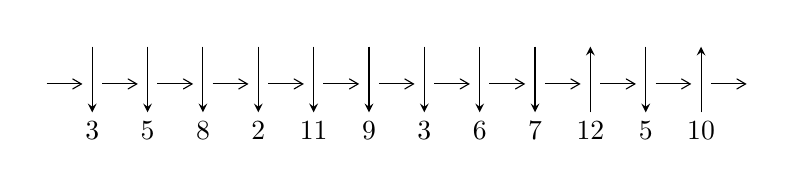
\begin{tikzpicture}[x=20pt, y=17pt]
	% nodes
	\node (C0) at (0, 0) {};
	\node (C1) at (1, 0) {};
	\node (C1U) at (1, +1) {};
	\node (C1D) at (1, -1) {3};

	\node (C2) at (2, 0) {};
	\node (C2U) at (2, +1) {};
	\node (C2D) at (2, -1) {5};

	\node (C3) at (3, 0) {};
	\node (C3U) at (3, +1) {};
	\node (C3D) at (3, -1) {8};

	\node (C4) at (4, 0) {};
	\node (C4U) at (4, +1) {};
	\node (C4D) at (4, -1) {2};

	\node (C5) at (5, 0) {};
	\node (C5U) at (5, +1) {};
	\node (C5D) at (5, -1) {11};

	\node (C6) at (6, 0) {};
	\node (C6U) at (6, +1) {};
	\node (C6D) at (6, -1) {9};

	\node (C7) at (7, 0) {};
	\node (C7U) at (7, +1) {};
	\node (C7D) at (7, -1) {3};

	\node (C8) at (8, 0) {};
	\node (C8U) at (8, +1) {};
	\node (C8D) at (8, -1) {6};

	\node (C9) at (9, 0) {};
	\node (C9U) at (9, +1) {};
	\node (C9D) at (9, -1) {7};

	\node (C10) at (10, 0) {};
	\node (C10U) at (10, +1) {};
	\node (C10D) at (10, -1) {12};

	\node (C11) at (11, 0) {};
	\node (C11U) at (11, +1) {};
	\node (C11D) at (11, -1) {5};

	\node (C12) at (12, 0) {};
	\node (C12U) at (12, +1) {};
	\node (C12D) at (12, -1) {10};
	\node (C13) at (13, 0) {};

	% arrows
	\draw[->,>={angle 60}]
	(C0) edge (C1) (C1) edge (C2) (C2) edge (C3) (C3) edge (C4) (C4) edge (C5) (C5) edge (C6) (C6) edge (C7) (C7) edge (C8) (C8) edge (C9) (C9) edge (C10) (C10) edge (C11) (C11) edge (C12) (C12) edge (C13) ;	\draw[->,>=stealth]
	(C1U) edge (C1D) (C2U) edge (C2D) (C3U) edge (C3D) (C4U) edge (C4D) (C5U) edge (C5D) (C6U) edge (C6D) (C7U) edge (C7D) (C8U) edge (C8D) (C9U) edge (C9D) (C10D) edge (C10U) (C11U) edge (C11D) (C12D) edge (C12U) ;
	\end{tikzpicture} \\
\hhline{~~} \\& 
\textbf{Solving Sequence} \\ \cline{2-2} 
 &
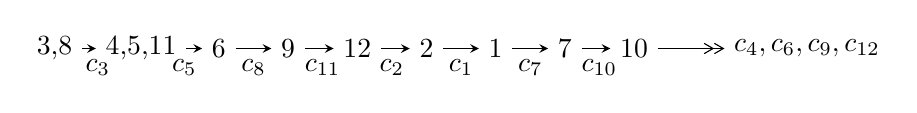
\begin{tikzpicture}[x=25pt, y=7pt]
	% node
	\node (A0) at (-1/8, 0) {3,8};
	\node (A1) at (9/8, 0) {4,5,11};
	\node (A2) at (9/4, 0) {6};
	\node (A3) at (13/4, 0) {9};
	\node (A4) at (17/4, 0) {12};
	\node (A5) at (21/4, 0) {2};
	\node (A6) at (25/4, 0) {1};
	\node (A7) at (29/4, 0) {7};
	\node (A8) at (33/4, 0) {10};
	\node (C1) at (1/2, -1) {$c_{3}$};
	\node (C2) at (7/4, -1) {$c_{5}$};
	\node (C3) at (11/4, -1) {$c_{8}$};
	\node (C4) at (15/4, -1) {$c_{11}$};
	\node (C5) at (19/4, -1) {$c_{2}$};
	\node (C6) at (23/4, -1) {$c_{1}$};
	\node (C7) at (27/4, -1) {$c_{7}$};
	\node (C8) at (31/4, -1) {$c_{10}$};
	\node (A9) at (43/4, 0) {$c_{4},c_{6},c_{9},c_{12}$};

	% edge
	\draw[->,>=stealth]	
	(A0) edge (A1) (A1) edge (A2) (A2) edge (A3) (A3) edge (A4) (A4) edge (A5) (A5) edge (A6) (A6) edge (A7) (A7) edge (A8) ;
	\draw[->>,>={angle 60}]	
	(A8) edge (A9);
\end{tikzpicture} \\ 

\end{tabular} \\

\footnotetext{
The image of knot diagram is generated by the software ``\textbf{Draw programme}" developed by Andrew Bartholomew(\url{http://www.layer8.co.uk/maths/draw/index.htm\#Running-draw}), where we modified some parts for our purpose(\url{https://github.com/CATsTAILs/LinksPainter}).
}\phantom \\ \newline 
\centering \textbf{Ideals for irreducible components\footnotemark of $X_{\text{par}}$} 
 
\begin{align*}
I^u_{1}&=\langle 
4.74944\times10^{17} u^{17}+1.40015\times10^{18} u^{16}+\cdots+6.24112\times10^{19} d-1.05622\times10^{18},\\
\phantom{I^u_{1}}&\phantom{= \langle  }-6.60139\times10^{16} u^{17}-1.14793\times10^{18} u^{16}+\cdots+1.24822\times10^{20} c+5.64891\times10^{19},\\
\phantom{I^u_{1}}&\phantom{= \langle  }-5.68457\times10^{17} u^{17}-8.64985\times10^{17} u^{16}+\cdots+1.24822\times10^{20} b-1.55459\times10^{19},\\
\phantom{I^u_{1}}&\phantom{= \langle  }2.99690\times10^{17} u^{17}+2.72458\times10^{17} u^{16}+\cdots+2.49645\times10^{20} a-2.46906\times10^{20},\;u^{18}+3 u^{17}+\cdots+32 u+32\rangle \\
I^u_{2}&=\langle 
6226 u^9 a+7765 u^9+\cdots-39596 a-22790,\;19798 u^9 a+1477 u^9+\cdots-86484 a-5134,\\
\phantom{I^u_{2}}&\phantom{= \langle  }1447 u^9 a+65 u^9+\cdots-7346 a-3206,\;-22391 u^9 a+7563 u^9+\cdots+121770 a-50482,\\
\phantom{I^u_{2}}&\phantom{= \langle  }u^{10}- u^9-7 u^8+8 u^7+13 u^6-14 u^5-2 u^4-2 u^3+13 u^2-12 u+4\rangle \\
\\
I^v_{1}&=\langle 
c,\;d+v,\;b,\;a-1,\;v^2- v+1\rangle \\
I^v_{2}&=\langle 
a,\;d+v,\;a v+c- v+1,\;b-1,\;v^2- v+1\rangle \\
I^v_{3}&=\langle 
a,\;d+1,\;c+a,\;b-1,\;v+1\rangle \\
I^v_{4}&=\langle 
a,\;d^2 a- d^2 v- d c+d v+d- v-1,\;d^2 v^2- v^2 d- d v+v^2+2 v+1,\\
\phantom{I^v_{4}}&\phantom{= \langle  }d c a- d c v- d a+d v- c^2+c v- a v+2 c- a-1,\;v^2 d c- v^2 d- v^2 c+v^2 a- c v+2 a v+a,\\
\phantom{I^v_{4}}&\phantom{= \langle  }d a v+d a- d v- c v- c+v+1,\;c^2 v^2- v^2 c a+a^2 v^2- c a v- v^2 c+2 a^2 v- v^2 a+a^2- a v+v^2,\;b-1\rangle \\
\end{align*}
\raggedright * 5 irreducible components of $\dim_{\mathbb{C}}=0$, with total 43 representations.\\
\raggedright * 1 irreducible components of $\dim_{\mathbb{C}}=1$ \\
\footnotetext{All coefficients of polynomials are rational numbers. But the coefficients are sometimes approximated in decimal forms when there is not enough margin.}
\newpage
\renewcommand{\arraystretch}{1}
\centering \section*{I. $I^u_{1}= \langle 4.75\times10^{17} u^{17}+1.40\times10^{18} u^{16}+\cdots+6.24\times10^{19} d-1.06\times10^{18},\;-6.60\times10^{16} u^{17}-1.15\times10^{18} u^{16}+\cdots+1.25\times10^{20} c+5.65\times10^{19},\;-5.68\times10^{17} u^{17}-8.65\times10^{17} u^{16}+\cdots+1.25\times10^{20} b-1.55\times10^{19},\;3.00\times10^{17} u^{17}+2.72\times10^{17} u^{16}+\cdots+2.50\times10^{20} a-2.47\times10^{20},\;u^{18}+3 u^{17}+\cdots+32 u+32 \rangle$}
\flushleft \textbf{(i) Arc colorings}\\
\begin{tabular}{m{7pt} m{180pt} m{7pt} m{180pt} }
\flushright $a_{3}=$&$\begin{pmatrix}1\\0\end{pmatrix}$ \\
\flushright $a_{8}=$&$\begin{pmatrix}0\\u\end{pmatrix}$ \\
\flushright $a_{4}=$&$\begin{pmatrix}1\\u^2\end{pmatrix}$ \\
\flushright $a_{5}=$&$\begin{pmatrix}-0.00120047 u^{17}-0.00109138 u^{16}+\cdots-0.0893825 u+0.989028\\0.00455413 u^{17}+0.00692973 u^{16}+\cdots+0.245124 u+0.124544\end{pmatrix}$ \\
\flushright $a_{11}=$&$\begin{pmatrix}0.000528863 u^{17}+0.00919651 u^{16}+\cdots+0.525376 u-0.452556\\-0.00760992 u^{17}-0.0224344 u^{16}+\cdots+0.469479 u+0.0169236\end{pmatrix}$ \\
\flushright $a_{6}=$&$\begin{pmatrix}-0.00389201 u^{17}-0.00712189 u^{16}+\cdots+1.21746 u+0.120580\\0.00251002 u^{17}+0.00451441 u^{16}+\cdots+1.02744 u+0.0384150\end{pmatrix}$ \\
\flushright $a_{9}=$&$\begin{pmatrix}0.00640203 u^{17}+0.0116363 u^{16}+\cdots-0.190018 u-0.0821645\\0.00251002 u^{17}+0.00451441 u^{16}+\cdots+1.02744 u+0.0384150\end{pmatrix}$ \\
\flushright $a_{12}=$&$\begin{pmatrix}0.0117438 u^{17}+0.0288644 u^{16}+\cdots-0.134994 u-0.795004\\0.00684312 u^{17}+0.0134766 u^{16}+\cdots+0.331617 u+0.354667\end{pmatrix}$ \\
\flushright $a_{2}=$&$\begin{pmatrix}-0.00120047 u^{17}-0.00109138 u^{16}+\cdots-0.0893825 u+0.989028\\-0.00756978 u^{17}-0.0124143 u^{16}+\cdots-0.287029 u-0.204865\end{pmatrix}$ \\
\flushright $a_{1}=$&$\begin{pmatrix}-0.00877025 u^{17}-0.0135056 u^{16}+\cdots-0.376412 u+0.784163\\-0.00756978 u^{17}-0.0124143 u^{16}+\cdots-0.287029 u-0.204865\end{pmatrix}$ \\
\flushright $a_{7}=$&$\begin{pmatrix}u\\u\end{pmatrix}$ \\
\flushright $a_{10}=$&$\begin{pmatrix}0.0131347 u^{17}+0.0229449 u^{16}+\cdots-0.168830 u+0.0635675\\0.00924267 u^{17}+0.0158230 u^{16}+\cdots+1.04863 u+0.184147\end{pmatrix}$\\&\end{tabular}
\flushleft \textbf{(ii) Obstruction class $= -1$}\\~\\
\flushleft \textbf{(iii) Cusp Shapes $= -\frac{1881106086253954753}{31205580083057755580} u^{17}-\frac{5887773742508132609}{62411160166115511160} u^{16}+\cdots-\frac{57261478582730965292}{7801395020764438895} u-\frac{64355080374530213256}{7801395020764438895}$}\\~\\
\newpage\renewcommand{\arraystretch}{1}
\flushleft \textbf{(iv) u-Polynomials at the component}\newline \\
\begin{tabular}{m{50pt}|m{274pt}}
Crossings & \hspace{64pt}u-Polynomials at each crossing \\
\hline $$\begin{aligned}c_{1}\end{aligned}$$&$\begin{aligned}
&u^{18}+29 u^{17}+\cdots+26 u+1
\end{aligned}$\\
\hline $$\begin{aligned}c_{2},c_{4},c_{6}\\c_{8},c_{9}\end{aligned}$$&$\begin{aligned}
&u^{18}-5 u^{17}+\cdots+2 u-1
\end{aligned}$\\
\hline $$\begin{aligned}c_{3},c_{7}\end{aligned}$$&$\begin{aligned}
&u^{18}-3 u^{17}+\cdots-32 u+32
\end{aligned}$\\
\hline $$\begin{aligned}c_{5},c_{11}\end{aligned}$$&$\begin{aligned}
&u^{18}- u^{17}+\cdots+12 u+4
\end{aligned}$\\
\hline $$\begin{aligned}c_{10},c_{12}\end{aligned}$$&$\begin{aligned}
&u^{18}-5 u^{17}+\cdots+136 u+16
\end{aligned}$\\
\hline
\end{tabular}\\~\\
\newpage\renewcommand{\arraystretch}{1}
\flushleft \textbf{(v) Riley Polynomials at the component}\newline \\
\begin{tabular}{m{50pt}|m{274pt}}
Crossings & \hspace{64pt}Riley Polynomials at each crossing \\
\hline $$\begin{aligned}c_{1}\end{aligned}$$&$\begin{aligned}
&y^{18}-69 y^{17}+\cdots-166 y+1
\end{aligned}$\\
\hline $$\begin{aligned}c_{2},c_{4},c_{6}\\c_{8},c_{9}\end{aligned}$$&$\begin{aligned}
&y^{18}-29 y^{17}+\cdots-26 y+1
\end{aligned}$\\
\hline $$\begin{aligned}c_{3},c_{7}\end{aligned}$$&$\begin{aligned}
&y^{18}-15 y^{17}+\cdots-2048 y+1024
\end{aligned}$\\
\hline $$\begin{aligned}c_{5},c_{11}\end{aligned}$$&$\begin{aligned}
&y^{18}+5 y^{17}+\cdots-136 y+16
\end{aligned}$\\
\hline $$\begin{aligned}c_{10},c_{12}\end{aligned}$$&$\begin{aligned}
&y^{18}+17 y^{17}+\cdots-38944 y+256
\end{aligned}$\\
\hline
\end{tabular}\\~\\
\newpage\flushleft \textbf{(vi) Complex Volumes and Cusp Shapes}
$$\begin{array}{c|c|c}  
\text{Solutions to }I^u_{1}& \I (\text{vol} + \sqrt{-1}CS) & \text{Cusp shape}\\
 \hline 
\begin{aligned}
u &= -1.078440 + 0.216619 I \\
a &= \phantom{-}0.492205 - 0.156710 I \\
b &= \phantom{-}0.844681 + 0.587317 I \\
c &= \phantom{-}1.077070 - 0.430910 I \\
d &= \phantom{-}1.068210 - 0.698024 I\end{aligned}
 & -3.61986 - 3.92600 I & -13.3379 + 5.7849 I \\ \hline\begin{aligned}
u &= -1.078440 - 0.216619 I \\
a &= \phantom{-}0.492205 + 0.156710 I \\
b &= \phantom{-}0.844681 - 0.587317 I \\
c &= \phantom{-}1.077070 + 0.430910 I \\
d &= \phantom{-}1.068210 + 0.698024 I\end{aligned}
 & -3.61986 + 3.92600 I & -13.3379 - 5.7849 I \\ \hline\begin{aligned}
u &= \phantom{-}0.709201 + 0.274453 I \\
a &= \phantom{-}0.515734 + 0.082365 I \\
b &= \phantom{-}0.890761 - 0.301961 I \\
c &= \phantom{-}0.436964 + 0.773316 I \\
d &= -0.097657 - 0.668363 I\end{aligned}
 & -3.12578 - 1.29944 I & -14.10514 + 0.79844 I \\ \hline\begin{aligned}
u &= \phantom{-}0.709201 - 0.274453 I \\
a &= \phantom{-}0.515734 - 0.082365 I \\
b &= \phantom{-}0.890761 + 0.301961 I \\
c &= \phantom{-}0.436964 - 0.773316 I \\
d &= -0.097657 + 0.668363 I\end{aligned}
 & -3.12578 + 1.29944 I & -14.10514 - 0.79844 I \\ \hline\begin{aligned}
u &= -0.610909 + 0.417338 I \\
a &= \phantom{-}0.768504 + 0.302779 I \\
b &= \phantom{-}0.126387 - 0.443779 I \\
c &= -0.48208 - 1.41304 I \\
d &= -0.884219 - 0.662050 I\end{aligned}
 & \phantom{-}1.20916 + 1.63680 I & -1.95124 - 5.83411 I \\ \hline\begin{aligned}
u &= -0.610909 - 0.417338 I \\
a &= \phantom{-}0.768504 - 0.302779 I \\
b &= \phantom{-}0.126387 + 0.443779 I \\
c &= -0.48208 + 1.41304 I \\
d &= -0.884219 + 0.662050 I\end{aligned}
 & \phantom{-}1.20916 - 1.63680 I & -1.95124 + 5.83411 I\\
 \hline 
 \end{array}$$\newpage$$\begin{array}{c|c|c}  
\text{Solutions to }I^u_{1}& \I (\text{vol} + \sqrt{-1}CS) & \text{Cusp shape}\\
 \hline 
\begin{aligned}
u &= \phantom{-}0.555399\phantom{ +0.000000I} \\
a &= \phantom{-}0.739573\phantom{ +0.000000I} \\
b &= \phantom{-}0.352132\phantom{ +0.000000I} \\
c &= -0.371975\phantom{ +0.000000I} \\
d &= \phantom{-}0.206595\phantom{ +0.000000I}\end{aligned}
 & -0.726383\phantom{ +0.000000I} & -14.1310\phantom{ +0.000000I} \\ \hline\begin{aligned}
u &= -0.072203 + 0.503217 I \\
a &= \phantom{-}1.330050 + 0.161709 I \\
b &= -0.259101 - 0.090079 I \\
c &= -0.46842 + 1.35904 I \\
d &= \phantom{-}0.650071 + 0.333845 I\end{aligned}
 & -0.39079 - 2.25423 I & -1.75748 + 3.62098 I \\ \hline\begin{aligned}
u &= -0.072203 - 0.503217 I \\
a &= \phantom{-}1.330050 - 0.161709 I \\
b &= -0.259101 + 0.090079 I \\
c &= -0.46842 - 1.35904 I \\
d &= \phantom{-}0.650071 - 0.333845 I\end{aligned}
 & -0.39079 + 2.25423 I & -1.75748 - 3.62098 I \\ \hline\begin{aligned}
u &= -1.83506 + 0.34828 I \\
a &= -1.318640 - 0.296832 I \\
b &= -1.72178 + 0.16248 I \\
c &= \phantom{-}0.10743 + 1.64261 I \\
d &= \phantom{-}0.76923 + 2.97688 I\end{aligned}
 & -11.72250 + 5.21750 I & -12.21552 - 2.94469 I \\ \hline\begin{aligned}
u &= -1.83506 - 0.34828 I \\
a &= -1.318640 + 0.296832 I \\
b &= -1.72178 - 0.16248 I \\
c &= \phantom{-}0.10743 - 1.64261 I \\
d &= \phantom{-}0.76923 - 2.97688 I\end{aligned}
 & -11.72250 - 5.21750 I & -12.21552 + 2.94469 I \\ \hline\begin{aligned}
u &= -1.70473 + 1.04671 I \\
a &= -0.961354 - 0.702659 I \\
b &= -1.67800 + 0.49555 I \\
c &= -0.21746 - 1.42452 I \\
d &= -1.86176 - 2.20079 I\end{aligned}
 & \phantom{-}19.5607 + 13.8899 I & -13.2954 - 6.2001 I\\
 \hline 
 \end{array}$$\newpage$$\begin{array}{c|c|c}  
\text{Solutions to }I^u_{1}& \I (\text{vol} + \sqrt{-1}CS) & \text{Cusp shape}\\
 \hline 
\begin{aligned}
u &= -1.70473 - 1.04671 I \\
a &= -0.961354 + 0.702659 I \\
b &= -1.67800 - 0.49555 I \\
c &= -0.21746 + 1.42452 I \\
d &= -1.86176 + 2.20079 I\end{aligned}
 & \phantom{-}19.5607 - 13.8899 I & -13.2954 + 6.2001 I \\ \hline\begin{aligned}
u &= -0.16477 + 2.05598 I \\
a &= \phantom{-}0.354039 - 0.009486 I \\
b &= \phantom{-}1.82253 + 0.07562 I \\
c &= -0.653183 - 0.249237 I \\
d &= -0.62005 + 1.30187 I\end{aligned}
 & -15.4858 - 3.5329 I & -13.90580 + 2.19457 I \\ \hline\begin{aligned}
u &= -0.16477 - 2.05598 I \\
a &= \phantom{-}0.354039 + 0.009486 I \\
b &= \phantom{-}1.82253 - 0.07562 I \\
c &= -0.653183 + 0.249237 I \\
d &= -0.62005 - 1.30187 I\end{aligned}
 & -15.4858 + 3.5329 I & -13.90580 - 2.19457 I \\ \hline\begin{aligned}
u &= \phantom{-}2.12691\phantom{ +0.000000I} \\
a &= -1.17023\phantom{ +0.000000I} \\
b &= -1.85453\phantom{ +0.000000I} \\
c &= \phantom{-}0.262059\phantom{ +0.000000I} \\
d &= -0.557378\phantom{ +0.000000I}\end{aligned}
 & -16.6053\phantom{ +0.000000I} & -15.4680\phantom{ +0.000000I} \\ \hline\begin{aligned}
u &= \phantom{-}1.91575 + 0.96837 I \\
a &= -0.965214 + 0.561225 I \\
b &= -1.77427 - 0.45020 I \\
c &= -0.245361 + 0.187449 I \\
d &= \phantom{-}0.651569 - 0.121506 I\end{aligned}
 & \phantom{-}18.1284 - 6.9769 I & -14.6320 + 1.8700 I \\ \hline\begin{aligned}
u &= \phantom{-}1.91575 - 0.96837 I \\
a &= -0.965214 - 0.561225 I \\
b &= -1.77427 + 0.45020 I \\
c &= -0.245361 - 0.187449 I \\
d &= \phantom{-}0.651569 + 0.121506 I\end{aligned}
 & \phantom{-}18.1284 + 6.9769 I & -14.6320 - 1.8700 I\\
 \hline 
 \end{array}$$\newpage\newpage\renewcommand{\arraystretch}{1}
\centering \section*{II. $I^u_{2}= \langle 6226 a u^{9}+7765 u^{9}+\cdots-3.96\times10^{4} a-2.28\times10^{4},\;1.98\times10^{4} a u^{9}+1477 u^{9}+\cdots-8.65\times10^{4} a-5134,\;1447 a u^{9}+65 u^{9}+\cdots-7346 a-3206,\;-2.24\times10^{4} a u^{9}+7563 u^{9}+\cdots+1.22\times10^{5} a-5.05\times10^{4},\;u^{10}- u^9+\cdots-12 u+4 \rangle$}
\flushleft \textbf{(i) Arc colorings}\\
\begin{tabular}{m{7pt} m{180pt} m{7pt} m{180pt} }
\flushright $a_{3}=$&$\begin{pmatrix}1\\0\end{pmatrix}$ \\
\flushright $a_{8}=$&$\begin{pmatrix}0\\u\end{pmatrix}$ \\
\flushright $a_{4}=$&$\begin{pmatrix}1\\u^2\end{pmatrix}$ \\
\flushright $a_{5}=$&$\begin{pmatrix}a\\-0.422112 a u^{9}-0.0189615 u^{9}+\cdots+2.14294 a+0.935239\end{pmatrix}$ \\
\flushright $a_{11}=$&$\begin{pmatrix}-1.44384 a u^{9}-0.107716 u^{9}+\cdots+6.30718 a+0.374417\\-0.908110 a u^{9}-1.13258 u^{9}+\cdots+5.77538 a+3.32410\end{pmatrix}$ \\
\flushright $a_{6}=$&$\begin{pmatrix}\frac{3673}{6856} u^9 a+\frac{1}{4} u^9+\cdots-\frac{1823}{3428} a-3\\1.03574 u^{9}-0.613623 u^{8}+\cdots+10.7148 u-6.53180\end{pmatrix}$ \\
\flushright $a_{9}=$&$\begin{pmatrix}-0.535735 a u^{9}+0.785735 u^{9}+\cdots+0.531797 a-3.53180\\1.03574 u^{9}-0.613623 u^{8}+\cdots+10.7148 u-6.53180\end{pmatrix}$ \\
\flushright $a_{12}=$&$\begin{pmatrix}-0.663652 a u^{9}-0.107716 u^{9}+\cdots+2.73337 a+0.374417\\-0.682614 a u^{9}-0.637544 u^{9}+\cdots+3.66861 a+1.89177\end{pmatrix}$ \\
\flushright $a_{2}=$&$\begin{pmatrix}a\\0.422112 a u^{9}+0.0189615 u^{9}+\cdots-2.14294 a-0.935239\end{pmatrix}$ \\
\flushright $a_{1}=$&$\begin{pmatrix}0.422112 a u^{9}+0.0189615 u^{9}+\cdots-1.14294 a-0.935239\\0.422112 a u^{9}+0.0189615 u^{9}+\cdots-2.14294 a-0.935239\end{pmatrix}$ \\
\flushright $a_{7}=$&$\begin{pmatrix}u\\u\end{pmatrix}$ \\
\flushright $a_{10}=$&$\begin{pmatrix}-0.681009 a u^{9}+0.785735 u^{9}+\cdots+2.22025 a-3.53180\\-0.145274 a u^{9}+1.03574 u^{9}+\cdots+1.68845 a-6.53180\end{pmatrix}$\\&\end{tabular}
\flushleft \textbf{(ii) Obstruction class $= -1$}\\~\\
\flushleft \textbf{(iii) Cusp Shapes $= -\frac{3875}{1714} u^9+\frac{183}{1714} u^8+\frac{26957}{1714} u^7-\frac{2248}{857} u^6-\frac{51811}{1714} u^5-\frac{541}{857} u^4+\frac{185}{857} u^3+\frac{9943}{857} u^2-\frac{27495}{1714} u-\frac{882}{857}$}\\~\\
\newpage\renewcommand{\arraystretch}{1}
\flushleft \textbf{(iv) u-Polynomials at the component}\newline \\
\begin{tabular}{m{50pt}|m{274pt}}
Crossings & \hspace{64pt}u-Polynomials at each crossing \\
\hline $$\begin{aligned}c_{1}\end{aligned}$$&$\begin{aligned}
&u^{20}+19 u^{19}+\cdots-1248 u+256
\end{aligned}$\\
\hline $$\begin{aligned}c_{2},c_{4},c_{6}\\c_{8},c_{9}\end{aligned}$$&$\begin{aligned}
&u^{20}-3 u^{19}+\cdots+8 u+16
\end{aligned}$\\
\hline $$\begin{aligned}c_{3},c_{7}\end{aligned}$$&$\begin{aligned}
&(u^{10}+u^9-7 u^8-8 u^7+13 u^6+14 u^5-2 u^4+2 u^3+13 u^2+12 u+4)^2
\end{aligned}$\\
\hline $$\begin{aligned}c_{5},c_{11}\end{aligned}$$&$\begin{aligned}
&(u^{10}-2 u^9+3 u^8-2 u^7+4 u^6-3 u^5+3 u^4+3 u^2- u+1)^2
\end{aligned}$\\
\hline $$\begin{aligned}c_{10},c_{12}\end{aligned}$$&$\begin{aligned}
&(u^{10}-2 u^9+9 u^8-14 u^7+28 u^6-31 u^5+35 u^4-20 u^3+15 u^2-5 u+1)^{2}
\end{aligned}$\\
\hline
\end{tabular}\\~\\
\newpage\renewcommand{\arraystretch}{1}
\flushleft \textbf{(v) Riley Polynomials at the component}\newline \\
\begin{tabular}{m{50pt}|m{274pt}}
Crossings & \hspace{64pt}Riley Polynomials at each crossing \\
\hline $$\begin{aligned}c_{1}\end{aligned}$$&$\begin{aligned}
&y^{20}-39 y^{19}+\cdots-4268544 y+65536
\end{aligned}$\\
\hline $$\begin{aligned}c_{2},c_{4},c_{6}\\c_{8},c_{9}\end{aligned}$$&$\begin{aligned}
&y^{20}-19 y^{19}+\cdots+1248 y+256
\end{aligned}$\\
\hline $$\begin{aligned}c_{3},c_{7}\end{aligned}$$&$\begin{aligned}
&(y^{10}-15 y^9+\cdots-40 y+16)^{2}
\end{aligned}$\\
\hline $$\begin{aligned}c_{5},c_{11}\end{aligned}$$&$\begin{aligned}
&(y^{10}+2 y^9+9 y^8+14 y^7+28 y^6+31 y^5+35 y^4+20 y^3+15 y^2+5 y+1)^{2}
\end{aligned}$\\
\hline $$\begin{aligned}c_{10},c_{12}\end{aligned}$$&$\begin{aligned}
&(y^{10}+14 y^9+\cdots+5 y+1)^{2}
\end{aligned}$\\
\hline
\end{tabular}\\~\\
\newpage\flushleft \textbf{(vi) Complex Volumes and Cusp Shapes}
$$\begin{array}{c|c|c}  
\text{Solutions to }I^u_{2}& \I (\text{vol} + \sqrt{-1}CS) & \text{Cusp shape}\\
 \hline 
\begin{aligned}
u &= -0.620250 + 0.748934 I \\
a &= \phantom{-}0.448932 - 0.060647 I \\
b &= \phantom{-}1.187590 + 0.295523 I \\
c &= -0.036785 + 1.027380 I \\
d &= \phantom{-}0.50487 + 1.48189 I\end{aligned}
 & -4.43566 + 1.46073 I & -14.6593 - 3.2864 I \\ \hline\begin{aligned}
u &= -0.620250 + 0.748934 I \\
a &= -0.77388 - 2.52919 I \\
b &= -1.110620 + 0.361536 I \\
c &= -0.84252 + 1.37187 I \\
d &= \phantom{-}0.746622 + 0.664780 I\end{aligned}
 & -4.43566 + 1.46073 I & -14.6593 - 3.2864 I \\ \hline\begin{aligned}
u &= -0.620250 - 0.748934 I \\
a &= \phantom{-}0.448932 + 0.060647 I \\
b &= \phantom{-}1.187590 - 0.295523 I \\
c &= -0.036785 - 1.027380 I \\
d &= \phantom{-}0.50487 - 1.48189 I\end{aligned}
 & -4.43566 - 1.46073 I & -14.6593 + 3.2864 I \\ \hline\begin{aligned}
u &= -0.620250 - 0.748934 I \\
a &= -0.77388 + 2.52919 I \\
b &= -1.110620 - 0.361536 I \\
c &= -0.84252 - 1.37187 I \\
d &= \phantom{-}0.746622 - 0.664780 I\end{aligned}
 & -4.43566 - 1.46073 I & -14.6593 + 3.2864 I \\ \hline\begin{aligned}
u &= \phantom{-}0.793271 + 0.121626 I \\
a &= \phantom{-}0.549929 + 0.112131 I \\
b &= \phantom{-}0.745831 - 0.355977 I \\
c &= -0.79610 - 1.70490 I \\
d &= -2.03769 - 3.21838 I\end{aligned}
 & -2.87696 + 2.81207 I & -12.88002 - 4.64391 I \\ \hline\begin{aligned}
u &= \phantom{-}0.793271 + 0.121626 I \\
a &= -4.13892 + 0.99173 I \\
b &= -1.228490 - 0.054749 I \\
c &= \phantom{-}3.11748 + 3.57912 I \\
d &= \phantom{-}0.42416 + 1.44928 I\end{aligned}
 & -2.87696 + 2.81207 I & -12.88002 - 4.64391 I\\
 \hline 
 \end{array}$$\newpage$$\begin{array}{c|c|c}  
\text{Solutions to }I^u_{2}& \I (\text{vol} + \sqrt{-1}CS) & \text{Cusp shape}\\
 \hline 
\begin{aligned}
u &= \phantom{-}0.793271 - 0.121626 I \\
a &= \phantom{-}0.549929 - 0.112131 I \\
b &= \phantom{-}0.745831 + 0.355977 I \\
c &= -0.79610 + 1.70490 I \\
d &= -2.03769 + 3.21838 I\end{aligned}
 & -2.87696 - 2.81207 I & -12.88002 + 4.64391 I \\ \hline\begin{aligned}
u &= \phantom{-}0.793271 - 0.121626 I \\
a &= -4.13892 - 0.99173 I \\
b &= -1.228490 + 0.054749 I \\
c &= \phantom{-}3.11748 - 3.57912 I \\
d &= \phantom{-}0.42416 - 1.44928 I\end{aligned}
 & -2.87696 - 2.81207 I & -12.88002 + 4.64391 I \\ \hline\begin{aligned}
u &= \phantom{-}0.413972 + 0.524496 I \\
a &= \phantom{-}0.920372 - 0.380673 I \\
b &= -0.072202 + 0.383745 I \\
c &= -1.62004 + 0.89776 I \\
d &= -0.357634 - 0.319019 I\end{aligned}
 & -1.39065 + 0.79591 I & -7.22040 + 0.81155 I \\ \hline\begin{aligned}
u &= \phantom{-}0.413972 + 0.524496 I \\
a &= \phantom{-}0.475648 + 0.039205 I \\
b &= \phantom{-}1.088210 - 0.172121 I \\
c &= \phantom{-}0.706375 - 0.124338 I \\
d &= \phantom{-}1.141520 + 0.478061 I\end{aligned}
 & -1.39065 + 0.79591 I & -7.22040 + 0.81155 I \\ \hline\begin{aligned}
u &= \phantom{-}0.413972 - 0.524496 I \\
a &= \phantom{-}0.920372 + 0.380673 I \\
b &= -0.072202 - 0.383745 I \\
c &= -1.62004 - 0.89776 I \\
d &= -0.357634 + 0.319019 I\end{aligned}
 & -1.39065 - 0.79591 I & -7.22040 - 0.81155 I \\ \hline\begin{aligned}
u &= \phantom{-}0.413972 - 0.524496 I \\
a &= \phantom{-}0.475648 - 0.039205 I \\
b &= \phantom{-}1.088210 + 0.172121 I \\
c &= \phantom{-}0.706375 + 0.124338 I \\
d &= \phantom{-}1.141520 - 0.478061 I\end{aligned}
 & -1.39065 - 0.79591 I & -7.22040 - 0.81155 I\\
 \hline 
 \end{array}$$\newpage$$\begin{array}{c|c|c}  
\text{Solutions to }I^u_{2}& \I (\text{vol} + \sqrt{-1}CS) & \text{Cusp shape}\\
 \hline 
\begin{aligned}
u &= \phantom{-}1.88200 + 0.46774 I \\
a &= -1.236340 + 0.360963 I \\
b &= -1.74531 - 0.21760 I \\
c &= -0.930133 + 0.846762 I \\
d &= -1.17593 + 1.51598 I\end{aligned}
 & -12.6890 - 7.4068 I & -12.74326 + 4.41038 I \\ \hline\begin{aligned}
u &= \phantom{-}1.88200 + 0.46774 I \\
a &= \phantom{-}0.385819 - 0.297883 I \\
b &= \phantom{-}0.623883 + 1.253760 I \\
c &= \phantom{-}0.399930 - 0.904911 I \\
d &= \phantom{-}2.14658 - 1.15854 I\end{aligned}
 & -12.6890 - 7.4068 I & -12.74326 + 4.41038 I \\ \hline\begin{aligned}
u &= \phantom{-}1.88200 - 0.46774 I \\
a &= -1.236340 - 0.360963 I \\
b &= -1.74531 + 0.21760 I \\
c &= -0.930133 - 0.846762 I \\
d &= -1.17593 - 1.51598 I\end{aligned}
 & -12.6890 + 7.4068 I & -12.74326 - 4.41038 I \\ \hline\begin{aligned}
u &= \phantom{-}1.88200 - 0.46774 I \\
a &= \phantom{-}0.385819 + 0.297883 I \\
b &= \phantom{-}0.623883 - 1.253760 I \\
c &= \phantom{-}0.399930 + 0.904911 I \\
d &= \phantom{-}2.14658 + 1.15854 I\end{aligned}
 & -12.6890 + 7.4068 I & -12.74326 - 4.41038 I \\ \hline\begin{aligned}
u &= -1.96899 + 0.18613 I \\
a &= -1.262570 - 0.138704 I \\
b &= -1.78259 + 0.08597 I \\
c &= -0.815769 + 0.005529 I \\
d &= -0.287282 + 0.794814 I\end{aligned}
 & -13.15130 + 0.50253 I & -13.49701 + 0.08773 I \\ \hline\begin{aligned}
u &= -1.96899 + 0.18613 I \\
a &= \phantom{-}0.381016 + 0.259317 I \\
b &= \phantom{-}0.79370 - 1.22078 I \\
c &= -0.182431 + 0.386420 I \\
d &= -1.60521 + 0.16272 I\end{aligned}
 & -13.15130 + 0.50253 I & -13.49701 + 0.08773 I\\
 \hline 
 \end{array}$$\newpage$$\begin{array}{c|c|c}  
\text{Solutions to }I^u_{2}& \I (\text{vol} + \sqrt{-1}CS) & \text{Cusp shape}\\
 \hline 
\begin{aligned}
u &= -1.96899 - 0.18613 I \\
a &= -1.262570 + 0.138704 I \\
b &= -1.78259 - 0.08597 I \\
c &= -0.815769 - 0.005529 I \\
d &= -0.287282 - 0.794814 I\end{aligned}
 & -13.15130 - 0.50253 I & -13.49701 - 0.08773 I \\ \hline\begin{aligned}
u &= -1.96899 - 0.18613 I \\
a &= \phantom{-}0.381016 - 0.259317 I \\
b &= \phantom{-}0.79370 + 1.22078 I \\
c &= -0.182431 - 0.386420 I \\
d &= -1.60521 - 0.16272 I\end{aligned}
 & -13.15130 - 0.50253 I & -13.49701 - 0.08773 I\\
 \hline 
 \end{array}$$\newpage\newpage\renewcommand{\arraystretch}{1}
\centering \section*{III. $I^v_{1}= \langle c,\;d+v,\;b,\;a-1,\;v^2- v+1 \rangle$}
\flushleft \textbf{(i) Arc colorings}\\
\begin{tabular}{m{7pt} m{180pt} m{7pt} m{180pt} }
\flushright $a_{3}=$&$\begin{pmatrix}1\\0\end{pmatrix}$ \\
\flushright $a_{8}=$&$\begin{pmatrix}v\\0\end{pmatrix}$ \\
\flushright $a_{4}=$&$\begin{pmatrix}1\\0\end{pmatrix}$ \\
\flushright $a_{5}=$&$\begin{pmatrix}1\\0\end{pmatrix}$ \\
\flushright $a_{11}=$&$\begin{pmatrix}0\\- v\end{pmatrix}$ \\
\flushright $a_{6}=$&$\begin{pmatrix}1\\v-1\end{pmatrix}$ \\
\flushright $a_{9}=$&$\begin{pmatrix}v-1\\- v+1\end{pmatrix}$ \\
\flushright $a_{12}=$&$\begin{pmatrix}v\\- v\end{pmatrix}$ \\
\flushright $a_{2}=$&$\begin{pmatrix}1\\0\end{pmatrix}$ \\
\flushright $a_{1}=$&$\begin{pmatrix}1\\0\end{pmatrix}$ \\
\flushright $a_{7}=$&$\begin{pmatrix}v\\0\end{pmatrix}$ \\
\flushright $a_{10}=$&$\begin{pmatrix}-1\\- v+1\end{pmatrix}$\\&\end{tabular}
\flushleft \textbf{(ii) Obstruction class $= 1$}\\~\\
\flushleft \textbf{(iii) Cusp Shapes $= 4 v-11$}\\~\\
\newpage\renewcommand{\arraystretch}{1}
\flushleft \textbf{(iv) u-Polynomials at the component}\newline \\
\begin{tabular}{m{50pt}|m{274pt}}
Crossings & \hspace{64pt}u-Polynomials at each crossing \\
\hline $$\begin{aligned}c_{1},c_{2},c_{3}\\c_{4},c_{7}\end{aligned}$$&$\begin{aligned}
&u^2
\end{aligned}$\\
\hline $$\begin{aligned}c_{5},c_{10}\end{aligned}$$&$\begin{aligned}
&u^2+u+1
\end{aligned}$\\
\hline $$\begin{aligned}c_{6}\end{aligned}$$&$\begin{aligned}
&(u-1)^2
\end{aligned}$\\
\hline $$\begin{aligned}c_{8},c_{9}\end{aligned}$$&$\begin{aligned}
&(u+1)^2
\end{aligned}$\\
\hline $$\begin{aligned}c_{11},c_{12}\end{aligned}$$&$\begin{aligned}
&u^2- u+1
\end{aligned}$\\
\hline
\end{tabular}\\~\\
\newpage\renewcommand{\arraystretch}{1}
\flushleft \textbf{(v) Riley Polynomials at the component}\newline \\
\begin{tabular}{m{50pt}|m{274pt}}
Crossings & \hspace{64pt}Riley Polynomials at each crossing \\
\hline $$\begin{aligned}c_{1},c_{2},c_{3}\\c_{4},c_{7}\end{aligned}$$&$\begin{aligned}
&y^2
\end{aligned}$\\
\hline $$\begin{aligned}c_{5},c_{10},c_{11}\\c_{12}\end{aligned}$$&$\begin{aligned}
&y^2+y+1
\end{aligned}$\\
\hline $$\begin{aligned}c_{6},c_{8},c_{9}\end{aligned}$$&$\begin{aligned}
&(y-1)^2
\end{aligned}$\\
\hline
\end{tabular}\\~\\
\newpage\flushleft \textbf{(vi) Complex Volumes and Cusp Shapes}
$$\begin{array}{c|c|c}  
\text{Solutions to }I^v_{1}& \I (\text{vol} + \sqrt{-1}CS) & \text{Cusp shape}\\
 \hline 
\begin{aligned}
v &= \phantom{-}0.500000 + 0.866025 I \\
a &= \phantom{-}1.00000\phantom{ +0.000000I} \\
b &= \phantom{-0.000000 } 0 \\
c &= \phantom{-0.000000 } 0 \\
d &= -0.500000 - 0.866025 I\end{aligned}
 & -1.64493 - 2.02988 I & -9.00000 + 3.46410 I \\ \hline\begin{aligned}
v &= \phantom{-}0.500000 - 0.866025 I \\
a &= \phantom{-}1.00000\phantom{ +0.000000I} \\
b &= \phantom{-0.000000 } 0 \\
c &= \phantom{-0.000000 } 0 \\
d &= -0.500000 + 0.866025 I\end{aligned}
 & -1.64493 + 2.02988 I & -9.00000 - 3.46410 I\\
 \hline 
 \end{array}$$\newpage\newpage\renewcommand{\arraystretch}{1}
\centering \section*{IV. $I^v_{2}= \langle a,\;d+v,\;a v+c- v+1,\;b-1,\;v^2- v+1 \rangle$}
\flushleft \textbf{(i) Arc colorings}\\
\begin{tabular}{m{7pt} m{180pt} m{7pt} m{180pt} }
\flushright $a_{3}=$&$\begin{pmatrix}1\\0\end{pmatrix}$ \\
\flushright $a_{8}=$&$\begin{pmatrix}v\\0\end{pmatrix}$ \\
\flushright $a_{4}=$&$\begin{pmatrix}1\\0\end{pmatrix}$ \\
\flushright $a_{5}=$&$\begin{pmatrix}0\\1\end{pmatrix}$ \\
\flushright $a_{11}=$&$\begin{pmatrix}v-1\\- v\end{pmatrix}$ \\
\flushright $a_{6}=$&$\begin{pmatrix}v\\0\end{pmatrix}$ \\
\flushright $a_{9}=$&$\begin{pmatrix}v\\0\end{pmatrix}$ \\
\flushright $a_{12}=$&$\begin{pmatrix}v-1\\-1\end{pmatrix}$ \\
\flushright $a_{2}=$&$\begin{pmatrix}1\\-1\end{pmatrix}$ \\
\flushright $a_{1}=$&$\begin{pmatrix}0\\-1\end{pmatrix}$ \\
\flushright $a_{7}=$&$\begin{pmatrix}v\\0\end{pmatrix}$ \\
\flushright $a_{10}=$&$\begin{pmatrix}v\\0\end{pmatrix}$\\&\end{tabular}
\flushleft \textbf{(ii) Obstruction class $= 1$}\\~\\
\flushleft \textbf{(iii) Cusp Shapes $= -4 v-7$}\\~\\
\newpage\renewcommand{\arraystretch}{1}
\flushleft \textbf{(iv) u-Polynomials at the component}\newline \\
\begin{tabular}{m{50pt}|m{274pt}}
Crossings & \hspace{64pt}u-Polynomials at each crossing \\
\hline $$\begin{aligned}c_{1},c_{2}\end{aligned}$$&$\begin{aligned}
&(u-1)^2
\end{aligned}$\\
\hline $$\begin{aligned}c_{3},c_{6},c_{7}\\c_{8},c_{9}\end{aligned}$$&$\begin{aligned}
&u^2
\end{aligned}$\\
\hline $$\begin{aligned}c_{4}\end{aligned}$$&$\begin{aligned}
&(u+1)^2
\end{aligned}$\\
\hline $$\begin{aligned}c_{5},c_{12}\end{aligned}$$&$\begin{aligned}
&u^2- u+1
\end{aligned}$\\
\hline $$\begin{aligned}c_{10},c_{11}\end{aligned}$$&$\begin{aligned}
&u^2+u+1
\end{aligned}$\\
\hline
\end{tabular}\\~\\
\newpage\renewcommand{\arraystretch}{1}
\flushleft \textbf{(v) Riley Polynomials at the component}\newline \\
\begin{tabular}{m{50pt}|m{274pt}}
Crossings & \hspace{64pt}Riley Polynomials at each crossing \\
\hline $$\begin{aligned}c_{1},c_{2},c_{4}\end{aligned}$$&$\begin{aligned}
&(y-1)^2
\end{aligned}$\\
\hline $$\begin{aligned}c_{3},c_{6},c_{7}\\c_{8},c_{9}\end{aligned}$$&$\begin{aligned}
&y^2
\end{aligned}$\\
\hline $$\begin{aligned}c_{5},c_{10},c_{11}\\c_{12}\end{aligned}$$&$\begin{aligned}
&y^2+y+1
\end{aligned}$\\
\hline
\end{tabular}\\~\\
\newpage\flushleft \textbf{(vi) Complex Volumes and Cusp Shapes}
$$\begin{array}{c|c|c}  
\text{Solutions to }I^v_{2}& \I (\text{vol} + \sqrt{-1}CS) & \text{Cusp shape}\\
 \hline 
\begin{aligned}
v &= \phantom{-}0.500000 + 0.866025 I \\
a &= \phantom{-0.000000 } 0 \\
b &= \phantom{-}1.00000\phantom{ +0.000000I} \\
c &= -0.500000 + 0.866025 I \\
d &= -0.500000 - 0.866025 I\end{aligned}
 & -1.64493 + 2.02988 I & -9.00000 - 3.46410 I \\ \hline\begin{aligned}
v &= \phantom{-}0.500000 - 0.866025 I \\
a &= \phantom{-0.000000 } 0 \\
b &= \phantom{-}1.00000\phantom{ +0.000000I} \\
c &= -0.500000 - 0.866025 I \\
d &= -0.500000 + 0.866025 I\end{aligned}
 & -1.64493 - 2.02988 I & -9.00000 + 3.46410 I\\
 \hline 
 \end{array}$$\newpage\newpage\renewcommand{\arraystretch}{1}
\centering \section*{V. $I^v_{3}= \langle a,\;d+1,\;c+a,\;b-1,\;v+1 \rangle$}
\flushleft \textbf{(i) Arc colorings}\\
\begin{tabular}{m{7pt} m{180pt} m{7pt} m{180pt} }
\flushright $a_{3}=$&$\begin{pmatrix}1\\0\end{pmatrix}$ \\
\flushright $a_{8}=$&$\begin{pmatrix}-1\\0\end{pmatrix}$ \\
\flushright $a_{4}=$&$\begin{pmatrix}1\\0\end{pmatrix}$ \\
\flushright $a_{5}=$&$\begin{pmatrix}0\\1\end{pmatrix}$ \\
\flushright $a_{11}=$&$\begin{pmatrix}0\\-1\end{pmatrix}$ \\
\flushright $a_{6}=$&$\begin{pmatrix}0\\1\end{pmatrix}$ \\
\flushright $a_{9}=$&$\begin{pmatrix}-1\\-1\end{pmatrix}$ \\
\flushright $a_{12}=$&$\begin{pmatrix}0\\-1\end{pmatrix}$ \\
\flushright $a_{2}=$&$\begin{pmatrix}1\\-1\end{pmatrix}$ \\
\flushright $a_{1}=$&$\begin{pmatrix}0\\-1\end{pmatrix}$ \\
\flushright $a_{7}=$&$\begin{pmatrix}-1\\0\end{pmatrix}$ \\
\flushright $a_{10}=$&$\begin{pmatrix}0\\-1\end{pmatrix}$\\&\end{tabular}
\flushleft \textbf{(ii) Obstruction class $= 1$}\\~\\
\flushleft \textbf{(iii) Cusp Shapes $= -12$}\\~\\
\newpage\renewcommand{\arraystretch}{1}
\flushleft \textbf{(iv) u-Polynomials at the component}\newline \\
\begin{tabular}{m{50pt}|m{274pt}}
Crossings & \hspace{64pt}u-Polynomials at each crossing \\
\hline $$\begin{aligned}c_{1},c_{2},c_{6}\end{aligned}$$&$\begin{aligned}
&u-1
\end{aligned}$\\
\hline $$\begin{aligned}c_{3},c_{5},c_{7}\\c_{10},c_{11},c_{12}\end{aligned}$$&$\begin{aligned}
&u
\end{aligned}$\\
\hline $$\begin{aligned}c_{4},c_{8},c_{9}\end{aligned}$$&$\begin{aligned}
&u+1
\end{aligned}$\\
\hline
\end{tabular}\\~\\
\newpage\renewcommand{\arraystretch}{1}
\flushleft \textbf{(v) Riley Polynomials at the component}\newline \\
\begin{tabular}{m{50pt}|m{274pt}}
Crossings & \hspace{64pt}Riley Polynomials at each crossing \\
\hline $$\begin{aligned}c_{1},c_{2},c_{4}\\c_{6},c_{8},c_{9}\end{aligned}$$&$\begin{aligned}
&y-1
\end{aligned}$\\
\hline $$\begin{aligned}c_{3},c_{5},c_{7}\\c_{10},c_{11},c_{12}\end{aligned}$$&$\begin{aligned}
&y
\end{aligned}$\\
\hline
\end{tabular}\\~\\
\newpage\flushleft \textbf{(vi) Complex Volumes and Cusp Shapes}
$$\begin{array}{c|c|c}  
\text{Solutions to }I^v_{3}& \I (\text{vol} + \sqrt{-1}CS) & \text{Cusp shape}\\
 \hline 
\begin{aligned}
v &= -1.00000\phantom{ +0.000000I} \\
a &= \phantom{-0.000000 } 0 \\
b &= \phantom{-}1.00000\phantom{ +0.000000I} \\
c &= \phantom{-0.000000 } 0 \\
d &= -1.00000\phantom{ +0.000000I}\end{aligned}
 & -3.28987\phantom{ +0.000000I} & -12.0000\phantom{ +0.000000I}\\
 \hline 
 \end{array}$$\newpage\newpage\renewcommand{\arraystretch}{1}
\centering \section*{VI. $I^v_{4}= \langle a,\;-d^{2} v+d v+\cdots+d-1,\;d^{2} v^{2}-d v^{2}+\cdots+2 v+1,\;-c d v+d v+\cdots-a-1,\;c d v^{2}-d v^{2}+\cdots+2 a v+a,\;a d v-d v+\cdots-c+1,\;c^{2} v^{2}-a c v^{2}+\cdots-a v+a^{2},\;b-1 \rangle$}
\flushleft \textbf{(i) Arc colorings}\\
\begin{tabular}{m{7pt} m{180pt} m{7pt} m{180pt} }
\flushright $a_{3}=$&$\begin{pmatrix}1\\0\end{pmatrix}$ \\
\flushright $a_{8}=$&$\begin{pmatrix}v\\0\end{pmatrix}$ \\
\flushright $a_{4}=$&$\begin{pmatrix}1\\0\end{pmatrix}$ \\
\flushright $a_{5}=$&$\begin{pmatrix}0\\1\end{pmatrix}$ \\
\flushright $a_{11}=$&$\begin{pmatrix}c\\d\end{pmatrix}$ \\
\flushright $a_{6}=$&$\begin{pmatrix}- c+1\\- d c+1\end{pmatrix}$ \\
\flushright $a_{9}=$&$\begin{pmatrix}c+v-1\\d c-1\end{pmatrix}$ \\
\flushright $a_{12}=$&$\begin{pmatrix}c\\d+c\end{pmatrix}$ \\
\flushright $a_{2}=$&$\begin{pmatrix}1\\-1\end{pmatrix}$ \\
\flushright $a_{1}=$&$\begin{pmatrix}0\\-1\end{pmatrix}$ \\
\flushright $a_{7}=$&$\begin{pmatrix}v\\0\end{pmatrix}$ \\
\flushright $a_{10}=$&$\begin{pmatrix}c-1\\d c-1\end{pmatrix}$\\&\end{tabular}
\flushleft \textbf{(ii) Obstruction class $= -1$}\\~\\
\flushleft \textbf{(iii) Cusp Shapes $= d^2 c- d^2-2 d c+v^2+4 c-15$}\\~\\
\flushleft \textbf{(iv) u-Polynomials at the component} : It cannot be defined for a positive dimension component.\\~\\
\flushleft \textbf{(v) Riley Polynomials at the component} : It cannot be defined for a positive dimension component.\\~\\
\newpage\flushleft \textbf{(iv) Complex Volumes and Cusp Shapes}
$$\begin{array}{c|c|c} 
\text{Solution to }I^v_{4}& \I (\text{vol} + \sqrt{-1}CS) & \text{Cusp shape}\\
 \hline 
\begin{aligned}
v &= \cdots \\
a &= \cdots \\
b &= \cdots \\
c &= \cdots \\
d &= \cdots\end{aligned}
 & -3.28987 + 2.02988 I & -12.35599 + 3.42923 I\\
 \hline 
 \end{array}
$$
\newpage\renewcommand{\arraystretch}{1}
\centering \section*{ VII. u-Polynomials}
\begin{tabular}{m{50pt}|m{274pt}}
Crossings & \hspace{64pt}u-Polynomials at each crossing \\
\hline $$\begin{aligned}c_{1}\end{aligned}$$&$\begin{aligned}
&u^2(u-1)^3(u^{18}+29 u^{17}+\cdots+26 u+1)\\
&\cdot(u^{20}+19 u^{19}+\cdots-1248 u+256)
\end{aligned}$\\
\hline $$\begin{aligned}c_{2},c_{6}\end{aligned}$$&$\begin{aligned}
&u^2(u-1)^3(u^{18}-5 u^{17}+\cdots+2 u-1)(u^{20}-3 u^{19}+\cdots+8 u+16)
\end{aligned}$\\
\hline $$\begin{aligned}c_{3},c_{7}\end{aligned}$$&$\begin{aligned}
&u^5(u^{10}+u^9+\cdots+12 u+4)^{2}\\
&\cdot(u^{18}-3 u^{17}+\cdots-32 u+32)
\end{aligned}$\\
\hline $$\begin{aligned}c_{4},c_{8},c_{9}\end{aligned}$$&$\begin{aligned}
&u^2(u+1)^3(u^{18}-5 u^{17}+\cdots+2 u-1)(u^{20}-3 u^{19}+\cdots+8 u+16)
\end{aligned}$\\
\hline $$\begin{aligned}c_{5},c_{11}\end{aligned}$$&$\begin{aligned}
&u(u^2- u+1)(u^2+u+1)\\
&\cdot(u^{10}-2 u^9+3 u^8-2 u^7+4 u^6-3 u^5+3 u^4+3 u^2- u+1)^2\\
&\cdot(u^{18}- u^{17}+\cdots+12 u+4)
\end{aligned}$\\
\hline $$\begin{aligned}c_{10}\end{aligned}$$&$\begin{aligned}
&u(u^2+u+1)^2\\
&\cdot(u^{10}-2 u^9+9 u^8-14 u^7+28 u^6-31 u^5+35 u^4-20 u^3+15 u^2-5 u+1)^{2}\\
&\cdot(u^{18}-5 u^{17}+\cdots+136 u+16)
\end{aligned}$\\
\hline $$\begin{aligned}c_{12}\end{aligned}$$&$\begin{aligned}
&u(u^2- u+1)^2\\
&\cdot(u^{10}-2 u^9+9 u^8-14 u^7+28 u^6-31 u^5+35 u^4-20 u^3+15 u^2-5 u+1)^{2}\\
&\cdot(u^{18}-5 u^{17}+\cdots+136 u+16)
\end{aligned}$\\
\hline
\end{tabular}\newpage\renewcommand{\arraystretch}{1}
\centering \section*{ VIII. Riley Polynomials}
\begin{tabular}{m{50pt}|m{274pt}}
Crossings & \hspace{64pt}Riley Polynomials at each crossing \\
\hline $$\begin{aligned}c_{1}\end{aligned}$$&$\begin{aligned}
&y^2(y-1)^3(y^{18}-69 y^{17}+\cdots-166 y+1)\\
&\cdot(y^{20}-39 y^{19}+\cdots-4268544 y+65536)
\end{aligned}$\\
\hline $$\begin{aligned}c_{2},c_{4},c_{6}\\c_{8},c_{9}\end{aligned}$$&$\begin{aligned}
&y^2(y-1)^3(y^{18}-29 y^{17}+\cdots-26 y+1)\\
&\cdot(y^{20}-19 y^{19}+\cdots+1248 y+256)
\end{aligned}$\\
\hline $$\begin{aligned}c_{3},c_{7}\end{aligned}$$&$\begin{aligned}
&y^5(y^{10}-15 y^9+\cdots-40 y+16)^{2}(y^{18}-15 y^{17}+\cdots-2048 y+1024)
\end{aligned}$\\
\hline $$\begin{aligned}c_{5},c_{11}\end{aligned}$$&$\begin{aligned}
&y(y^2+y+1)^2\\
&\cdot(y^{10}+2 y^9+9 y^8+14 y^7+28 y^6+31 y^5+35 y^4+20 y^3+15 y^2+5 y+1)^{2}\\
&\cdot(y^{18}+5 y^{17}+\cdots-136 y+16)
\end{aligned}$\\
\hline $$\begin{aligned}c_{10},c_{12}\end{aligned}$$&$\begin{aligned}
&y(y^2+y+1)^2(y^{10}+14 y^9+\cdots+5 y+1)^{2}\\
&\cdot(y^{18}+17 y^{17}+\cdots-38944 y+256)
\end{aligned}$\\
\hline
\end{tabular}
\vskip 2pc
\end{document}